\chapter{Methodology}
\label{ch:method}

\section{Overview}
This chapter explains how the dataset was built, how features were created from the ZHVI time series and ACS data, and how the machine learning models were trained and evaluated. Everything was done in Python using libraries like \texttt{pandas}, \texttt{scikit-learn}, and \texttt{matplotlib}. The whole goal was to set things up in a way that avoided target leakage and helped each model make useful predictions based only on information available at the time.

\section{Data collection and cleaning}
The main dataset came from Zillow’s Home Value Index (ZHVI), which contains monthly home value estimates for U.S. ZIP codes. We filtered it to only include rows from Georgia and cleaned the data to fix missing values in the \texttt{Metro} and \texttt{City} columns. ZIP codes with long gaps in the time series (over 12 months) were excluded.

We also pulled annual ACS 1-Year Estimates from the U.S. Census Bureau’s API. These included variables related to education, poverty, transportation access, household structure, and age breakdowns, aggregated at the county level. Since ACS doesn’t report at the ZIP level, each ZIP inherited the demographic data from its county and year.

\section{Feature engineering}
\subsection{Zillow-derived features}
For each ZIP and year, we generated time-based features from the historical ZHVI data leading up to that year. These included:
\begin{itemize}
    \item \textbf{FinalZHVI}: the home value at the end of the year.
    \item \textbf{AvgMonthlyGrowth}: average monthly percentage growth across the year.
    \item \textbf{Volatility}: standard deviation of monthly growth rates.
    \item \textbf{CAGR}: compound annual growth rate from the earliest available data point to the cutoff.
    \item \textbf{NegativeGrowthYears}: total number of years that showed negative YoY growth up to that point.
    \item \textbf{YoY\_LastYear}: percent growth from the previous year to the current one.
\end{itemize}

The target variable, \texttt{YoY\_target}, was the year-over-year growth from the current year to the next — for example, a row for 2016 would have 2017's YoY as the target.

\subsection{ACS features}
ACS data was merged by \texttt{CountyName} and \texttt{Year}, and included:
\begin{itemize}
    \item Percent of renters, households without a vehicle, and people in poverty.
    \item Education rates (bachelor’s degree or higher).
    \item Unemployment rate.
    \item Household sizes (1-person, 4+ people).
    \item Percent of population in age ranges 0--17, 18--34, and 65+.
\end{itemize}

This helped give context to each ZIP’s housing behavior based on local conditions.

\section{Dataset preparation}
After merging, we grouped rare counties and metro areas into an \texttt{Other} category to avoid overfitting. Categorical variables were one-hot encoded. Rows with missing target values were dropped, and the final dataset contained 3{,}009 rows and 139 columns.

To avoid data leakage, we did the train/test split by ZIP code. That way, if a ZIP appeared in training data, it wouldn’t appear in the test set, even across years.

\section{Feature selection}
We applied two methods to rank features:
\begin{itemize}
    \item \textbf{F-Regression:} Based on linear correlation between each feature and the target.
    \item \textbf{Mutual Information:} Captures any kind of dependency (not just linear).
\end{itemize}

Both methods were used to compare which features were most informative. These rankings were then used to build models with varying numbers of top features (from 1 to 50), and we compared performance using 3-fold cross-validation.

\begin{figure}[!ht]
    \centering
    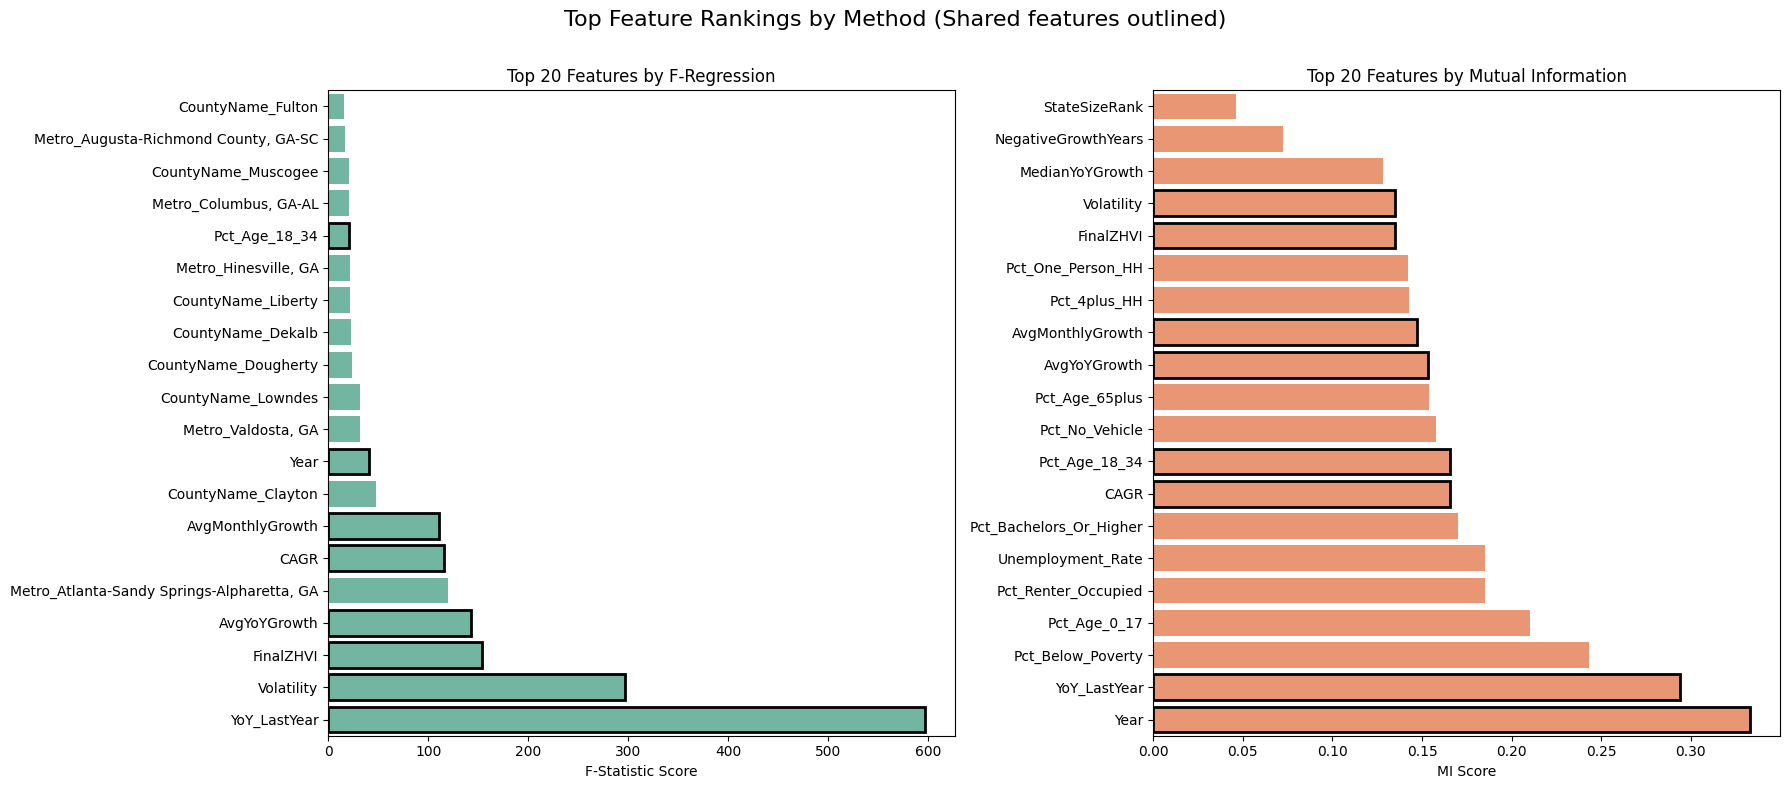
\includegraphics[width=\textwidth]{figures/topfeatures.png}
    \caption{Top 20 features by F-Regression and Mutual Information.}
    \label{fig:top_features}
\end{figure}
\FloatBarrier

Figure~\ref{fig:top_features} shows the top 20 features ranked by both methods. The most influential features were consistent across methods and included \texttt{YoY\_LastYear}, \texttt{Volatility}, \texttt{FinalZHVI}, and \texttt{AvgMonthlyGrowth}. F-regression emphasized time series performance metrics more strongly, while mutual information also highlighted ACS-derived features like poverty rate, vehicle access, and education level. This suggests that both price behavior and socioeconomic context contribute meaningfully to housing growth prediction.

\section{Model training and evaluation}
We tested three regression models:
\begin{itemize}
    \item Decision Tree Regressor,
    \item K-Nearest Neighbors (KNN),
    \item Random Forest Regressor.
\end{itemize}

Each model was tuned using \texttt{GridSearchCV}. The evaluation metrics included:
\begin{itemize}
    \item $R^2$ (coefficient of determination),
    \item RMSE (root mean squared error),
    \item MAE (mean absolute error),
    \item SMAPE (symmetric mean absolute percentage error).
\end{itemize}

Model performance was measured on a held-out test set of ZIP codes. Final evaluation included both numeric metrics and visual inspection via scatter plots and prediction-over-time charts.

\section{Ethical considerations}
This project uses only public datasets with no individual or sensitive personal data. All ACS data is aggregated at the county level, and ZHVI does not contain identifiable information. As such, no informed consent, privacy measures, or risk mitigation were needed. The model is intended for research and educational purposes and does not make real estate recommendations or financial decisions for individuals.

\section{Summary}
We started by cleaning and merging housing and demographic data. After engineering features and merging datasets, we created a ZIP–year format suitable for supervised learning. We used two feature selection methods to reduce dimensionality, and trained three different models with hyperparameter tuning and ZIP-based splits. Results were evaluated both quantitatively and visually to understand how well each model performed and where they differed.
